%&../settings/preamble.main

\ifsubfile
\usepackage[newfloat, cachedir=_minted-cache, outputdir=../build]{minted}
\usepackage{../libraries/set-minted}
\mintedpath{{../assets/codes/04/}}

\pagestyle{plain}
\setcounter{chapter}{3}

% arara: pdflatex: { options: ["--output-directory=../build"], shell: yes, draft: yes, synctex: no }
% arara: pdflatex: { options: ["--output-directory=../build"], shell: yes, synctex: no }
\begin{document}
\fi
\chapter{Strutture dati}
\epigraph{``Picking the wrong data structure for the job can be disastrous in terms of performance.
		    Identifying the very best data structure is usually not as critical, because there can be several choices that perform similarly.''}%
		 {--- \textup{\textsc{Steven S.\ Skiena, The Algorithm Design Manual (1997)}}}

\section{Strutture dati astratte}

\begin{definition}[Tipo di dato]
In un linguaggio di programmazione, un dato è un valore che una variabile può assumere.
\end{definition}

\begin{definition}[Tipo di dato astratto]
Un modello matematico, dato da una collezione di valori e un insieme di operazioni ammesse su questi valori.
\end{definition}

\begin{definition}[Tipi di dato primitivi]
Sono dei tipi di dati che vengono forniti direttamente dal linguaggio.
Come ad esempio: int (\texttt{+,-,*,/, \%}), boolean (\texttt{!, \&\&, ||}).
\end{definition}

Ogni tipo di dato deve distinguere \emph{specifica} ed \emph{implementazione} di un tipo di dato astratto.
La \emph{specifica} è astratta, il \enquote{manuale d'uso} che nasconde i dettagli implementativi all'utente, mentre l'\emph{implementazione} è la realizzazione vera e propria del tipo di dato.

\begin{table}[H]
	\centering
	\caption{Differenza fra specifica ed implementazione}
	\label{tab:differenza-specifica-implementazione}
	\begin{tabular}{@{} *{2}{l} @{}}
		\toprule
			Specifica & Implementazione \\
		\midrule
			Numeri reali & IEEE-754\\
		\addlinespace
			\multirow{2}{*}{Pile} & Pile basate su vettori\\
								  & Pile basate su puntatori\\
	    \addlinespace
			\multirow{2}{*}{Code} & Code basate su vettori circolari\\
								  & Code basate su puntatori\\
		\bottomrule
	\end{tabular}
\end{table}

\begin{definition}[Strutture di dati]
Le strutture di dati sono collezioni di dati, caratterizzate più dall'organizzazione della collezione piuttosto che dal tipo dei dati in esse contenute.
\end{definition}

Le strutture dati sono un modo sistematico per organizzare i dati e su di esse sono definite un insieme di operatori che permettono di manipolare la struttura stessa.
Le strutture dati possono essere caratterizzate in vari modi:
\begin{itemize}
	\item \emph{lineari}/\emph{non lineari}: presentano (o meno) una sequenza al loro interno;
	\item \emph{statiche}/\emph{dinamiche}: possono variare (o meno) di dimensione o di contenuto;
	\item \emph{omogenee}/\emph{disomogenee}: si riferisce ai dati contenuti al loro interno.
\end{itemize}

\begin{table}[H]
	\centering
	\caption[Implementazione delle strutture dati nei vari linguaggi]{Implementazione delle strutture dati nei vari linguaggi.\\Nota che Java distingue chiaramente la specifica dall'implementazione}
	\label{tab:strutture-dati}
	\begin{tabular}{@{} l >{\ttfamily}l >{\ttfamily}l >{\ttfamily}l @{}}
	\toprule
		Tipo & \normalfont{Java} & \normalfont{\texttt{C++}} & \normalfont{Python} \\
	\midrule
		Sequenze & \makecell[l]{\alert{List, Queue, Deque},\\LinkedList, ArrayList,\\Stack, ArrayDeque} & \makecell[l]{list, forward\_list,\\vector, stack,\\queue, dequeue} & \makecell[l]{list,\\tuple}\\
	\midrule
		Insiemi & \makecell[l]{\alert{Set},\\TreeSet, HashSet,\\LinkedHashSet} & \makecell[l]{set,\\unordered\_set} & \makecell[l]{set,\\fronzenset}\\
	\midrule
		Dizionari & \makecell[l]{\alert{Map},\\HashTree, HashMap,\\LinkedHashMap} & \makecell[l]{map,\\unordered\_map} & \makecell[l]{dict}\\
	\midrule
		Alberi & \makecell[cc]{-} & \makecell[cc]{-} & \makecell[cc]{-}\\
	\midrule
		Grafi  & \makecell[cc]{-} & \makecell[cc]{-} & \makecell[cc]{-}\\
	\bottomrule
	\end{tabular}
\end{table}

\section{Sequenza}

Una sequenza è una struttura dati \emph{dinamica}, \emph{lineare} che rappresenta una sequenza \emph{ordinata} di valori, dove un valore può comparire più di una volta.
L'ordine all'interno della sequenza è importante.

Le operazioni ammesse su una sequenza sono:
\begin{itemize}
	\item L'aggiunta e la rimozione elementi, specificando la posizione (tipicamente un intero), l'elemento \(s_1\) si trova in posizione \({pos}_i\) ed esistono posizioni fittizie \({pos}_0\) e \({pos}_{n+1}\);
	\item Accesso diretto alla testa e coda;
	\item Accesso sequenziale a tutti gli altri elementi.
\end{itemize}

\begin{algorithm}[H]
	\caption[Specifica sequenza]{Specifica \textsc{Sequence}}
	%&../preamble

% arara: pdflatex: { synctex: no }
% arara: latexmk: { clean: partial }
\ifstandalone
\begin{document}
\begin{algorithm}[H]
\fi
\begin{minipage}[t]{.48\textwidth}

Una struttura dati \emph{dinamica}, \emph{lineare} che rappresenta una sequenza \emph{ordinata} di valori, dove lo stesso valore può comparire più volte.

\BlankLine
\sequenceConstructor

\BlankLine
\tcp{INTERPRETARE}
\Bool \listEmpty \Comment*[r]{\True se la sequenza è vuota}
\Bool \listEnd \Comment*[r]{\True se \(p\) è uguale a \(pos_0\) o a \(pos_{n+1}\)}

\BlankLine
\tcp{LEGGERE}
\Pos \listHead \Comment*[r]{posizione del primo elemento}
\Pos \listTail \Comment*[r]{posizione dell'ultimo elemento}

\BlankLine
\tcp{ITERARE}
\Pos \listSucc \Comment*[r]{posizione dell'elem.\ che segue \(p\)}
\Pos \listPred \Comment*[r]{posizione dell'elem.\ che precede \(p\)}

% \vspace{20pt}
\end{minipage}\hfill%
\begin{minipage}[t]{.45\textwidth}

% \BlankLine
\tcp{MODIFICA}

\BlankLine
\tcp{inserisce l'elemento di tipo \Item nella posizione \(p\),}
\tcp{ritorna la nuova posizione,}
\tcp{che diviene il predecessore di \(p\)}
\Pos \listInsert{\Pos p, \Item v}

\tcp{rimuove l'elemento contenuto nella pos.\ \(p\),}
\tcp{ritorna il successore di \(p\)}
\Pos \listRemove{\Pos p}

\BlankLine
\tcp{legge l'elemento di tipo \Item}
\tcp{contenuto nella posizione \(p\)}
\listRead{\Pos p}

\BlankLine
\tcp{scrive l'elemento \(v\) di tipo \Item}
\tcp{nella posizione \(p\)}
\listWrite{\Pos p, \Item v}

\vphantom{0pt}
\end{minipage}
\ifstandalone
\end{algorithm}
\end{document}
\fi

\end{algorithm}

\clearpage
\subsection{Implementazione delle sequenze}

Di seguito vengono presentati alcuni esempi d'utilizzo dell'implementazione delle sequenze nei diversi linguaggi di programmazione utilizzati oggigiorno.

\begin{code}
\captionof{listing}{Implementazione delle liste in Java}
% \label{code:java-sequence}
\begin{minted}{java}
List<String> lista = new LinkedList<String>();
lista.add("two");
lista.addFirst("one");
lista.addLast("three");

Result: [ "one", "two", "three" ]
\end{minted}
\end{code}

\begin{code}
\captionof{listing}{Implementazione delle liste in \texttt{C++}}
% \label{code:cpp-sequence}
\begin{minted}{cpp}
std::list<int> lista;
lista.push_front(2);
lista.push_front(1);
lista.push_back(3);

Result: [1,2,3]
\end{minted}
\end{code}

\begin{code}
\captionof{listing}{Implementazione delle liste in Python}
% \label{code:python-sequence}
\begin{minted}{python}
lista = ["one", "three"]
lista.insert(1, "two")

Result: [ 'one', 'two', 'three' ]
\end{minted}
\end{code}

\section{Insiemi}

Un insieme è una struttura dati \emph{dinamica}, \emph{non lineare} che memorizza una \emph{collezione non ordinata di elementi} senza valori ripetuti.
L'ordinamento fra elementi è dato dall'eventuale relazione d'ordine definita sul tipo degli elementi stessi.

Le operazioni ammesse su un'insieme sono:
\begin{itemize}
	\item operazioni di base: come inserimento, cancellazione e verifica di contenimento;
	\item operazione di ordinamento: massimo, minimo;
	\item operazioni insiemistiche: unione, intersezione, differenza;
	\item iteratori: effettuare operazione per ogni elemento contenuto nell'insieme.
\end{itemize}

\begin{algorithm}[H]
	\caption[Struttura dati insieme]{Struttura dati \textsc{Set}}
	%&../preamble

% arara: pdflatex: { synctex: no }
% arara: latexmk: { clean: partial }
\ifstandalone
\begin{document}
\begin{algorithm}[H]
\fi
\begin{minipage}[t]{.45\textwidth}

Una struttura dati \emph{dinamica}, \emph{non lineare} che memorizza una \emph{collezione non ordinata di elementi} senza valori ripetuti.

\BlankLine
\setConstructor

\BlankLine
\tcp{INTERPRETARE}
\Int \setSize \Comment*[r]{cardinalità dell'insieme}
\Bool \setContains \Comment*[r]{\True se \(x\) è contenuto}

% \vspace{20pt}
\end{minipage}\hfill%
\begin{minipage}[t]{.48\textwidth}

% \BlankLine
\tcp{OPERAZIONI DI BASE}
\tcp{inserisce \(x\) nell'insieme, se assente}
\setInsert{\Item \(k\)}

\tcp{rimuove \(x\) nell'insieme, se presente}
\setRemove{\Item \(k\)}

\BlankLine
\tcp{OPERAZIONI INSIEMISTICHE}
\static \Set \setUnion{\Set \(A\), \Set \(B\)}\;
\static \Set \setIntersection{\Set \(A\), \Set \(B\)}\;
\static \Set \setDifference{\Set \(A\), \Set \(B\)}\;

\end{minipage}
\ifstandalone
\end{algorithm}
\end{document}
\fi

\end{algorithm}

\begin{code}
\captionof{listing}{Implementazione degli insiemi in Java}
% \label{code:java-set}
\begin{minted}{java}
List<String> lista = new LinkedList<String>();
Set<String> docenti = new TreeSet<>();
docenti.add("Alberto");
docenti.add("Cristian");
docenti.add("Alessio");

Result: { "Alberto", "Alessio", "Cristian" }
\end{minted}
\end{code}

\begin{code}
\captionof{listing}{Implementazione degli insiemi in \texttt{C++}}
% \label{code:cpp-set}
\begin{minted}{cpp}
std::set<std::string> frutta;
frutta.insert("mele");
frutta.insert("pere");
frutta.insert("banane");
frutta.insert("mele");
frutta.remove("mele")

Result: { "banane", "pere" }
\end{minted}
\end{code}

\begin{code}
\captionof{listing}{Implementazione degli insiemi in Python}
% \label{code:python-set}
\begin{minted}{python}
items = { "rock", "paper", "scissors", "rock" }
print(items)
print("Spock" in items)
print("lizard" not in items)

Result: { "rock", "paper", "scissors" }
False
True
\end{minted}
\end{code}

\section{Dizionari}

Un dizionario è una struttura dati che rappresenta il concetto matematico di \emph{relazione univoca} \(R : D \to C\), o associazione chiave-valore, dove:
\begin{itemize}
	\item l'insieme \(D\) è il dominio (gli elementi sono detti \emph{chiavi});
	\item l'insieme \(C\) è il codominio (gli elementi sono detti \emph{valori}).
\end{itemize}

Le operazioni ammesse sui dizionari sono:
\begin{itemize}
	\item ottenere il valore associato ad una particolare chiave (se presente) o \Nil se assente;
	\item inserire una nuova associazione chiave-valore, cancellando eventuali associazioni precedenti per la stessa chiave;
	\item rimuovere un'associazione chiave-valore esistente.
\end{itemize}

\begin{algorithm}[H]
	\caption[Specifica dizionario]{Specifica \textsc{Dictionary}}
	%&../preamble

% arara: pdflatex: { synctex: no }
% arara: latexmk: { clean: partial }
\ifstandalone
\begin{document}
\begin{algorithm}[H]
\fi

Un dizionario è una struttura dati che rappresenta il concetto matematico di \emph{relazione univoca} o associazione chiave-valore.

\BlankLine
\dictionaryConstructor

\BlankLine
\Item \dictLookup{\Item \(k\)} \Comment*[r]{restituisce il valore associato alla chiave \(k\), \Nil altrimenti}
\Item \dictInsert{\Key \(k\), \Item \(v\)} \Comment*[r]{associa il valore \(v\) alla chiave \(k\)}
\dictRemove{\Key \(k\)} \Comment*[r]{rimuove l'associazione della chiave \(k\)}

\ifstandalone
\end{algorithm}
\end{document}
\fi

\iffalse
% NOTE definizione alternativa
Struttura dati \emph{dinamica}, \emph{non lineare} che memorizza una collezione non ordinata di elementi senza valori ripetuti.
Rappresenta i concetto matematico di \emph{relazione univoca} \(R\colon D \to C\), o associazione chiave-valore. Dove \(D\) rappresenta il dominio di elementi detti \emph{chiave}, mentre \(C\) rappresenta il codominio degli elementi detti \emph{valori}.
Ogni \emph{valore} può essere associato a più \emph{chiavi}, ma non il contrario.

\BlankLine
\Item \dictLookup{\Item k} \Comment*[r]{restituisce il valore associato alla chiave \(k\) se presente, \Nil altrimenti}

\dictInsert{\Item k, \Item v} \Comment*[r]{associa il valore \(v\) alla chiave \(k\), sovrascrive se già presente}

\dictRemove{\Item k} \Comment*[r]{rimuove l'associazione della chiave \(k\)}
\fi

\end{algorithm}

\begin{code}
\captionof{listing}{Implementazione dei dizionari in Java}
% \label{code:java-liste}
\begin{minted}{java}
Map<String, String> capoluoghi = new HashMap<>();
capoluoghi.put("Toscana", "Firenze");
capoluoghi.put("Lombardia", "Milano");
capoluoghi.put("Sardegna", "Cagliari");
\end{minted}
\end{code}

\begin{code}
\captionof{listing}{Implementazione dei dizionari in \texttt{C++}}
% \label{code:cpp-liste}
\begin{minted}{cpp}
std::map<std::string, int> wordcounts;
std::string s;

while (std::cin >> s && s != "end")
  ++wordcounts[s];
\end{minted}
\end{code}

\begin{code}
\captionof{listing}{Implementazione dei dizionari in Python}
% \label{code:python-liste}
\begin{minted}{python}
v = {}
v[10] = 5
v["alberto"] = 42
v[10]+v["alberto"]

Result: 47
\end{minted}
\end{code}

\section{Alberi}

Un albero ordinato è dato da un insieme finito di elementi detti nodi.
Uno di questi nodi è designato come radice.
I rimanenti nodi, se esistono sono partizionati in insiemi \emph{ordinati} e \emph{disgiunti}, anch'essi alberi ordinati.

\begin{figure}[H]
	\centering
	\begin{forest} circled, wide
	[A
		[B[C]]
		[C[F][G]]
		[D[H][I]]
	]
	\end{forest}
	\caption[]{Un albero}
\end{figure}

Non vedremo implementazioni nei vari linguaggi in quanto non esiste una struttura dati definita riconosciuta universalmente.

\section{Grafi}

La struttura dati grafo è composta da:
\begin{itemize}
	\item un insieme di elementi detti nodi o vertici;
	\item un insieme di coppie (ordinate oppure no) di nodi detti archi.
\end{itemize}

% TODO inserire l'immagine di un grafo semplice

Tutte le operazioni su alberi e grafi ruotano attorno alla possibilità di effettuare visite su di essi, vedremo la specifica completa più avanti.

\begin{note}
La scelta della struttura dati si riflette sull'efficienza e sulle operazioni ammesse.
\end{note}

\clearpage
\section{Implementazione strutture dati elementari}

\subsection{Lista}

Una lista è una sequenza di nodi, contenenti dati arbitrari e 1-2 puntatori all'elemento successivo e/o precedente.

La contiguità nella lista non implica che ci sia continuità nella memoria.
Tutte le operazioni effettuate sulla lista hanno complessità \(\Omicron(1)\), ma per fare una ricerca dobbiamo spendere \(\Omicron(n)\).

Esistono diverse implmentazioni della lista, le quali possono essere:
\begin{itemize}
	\item bidirezionale o monodirezionale;
	\item con sentinella o senza;
	\item circolare o non circolare.
\end{itemize}

% TODO inserire immagine delle liste (da fare)

\begin{algorithm}[H]
	\caption{Struttura dati lista bidirezionale con sentinella in pseudocodice}
	%&../preamble

% arara: pdflatex: { synctex: no }
% arara: latexmk: { clean: partial }
\ifstandalone
\begin{document}
\begin{algorithm}[H]
\fi
\begin{minipage}[t]{.48\textwidth}

% \BlankLine
\List \Comment*[r]{bidirezionale con sentinella}

\BlankLine
\List \Pred		\Comment*[r]{predecessore}
\List \Succ		\Comment*[r]{successore}
\List \Value	\Comment*[r]{elemento}

\BlankLine
\prototype{\List \listConstructor}{
	\tcp{la sentinella fa riferimento a sé stessa}
	\(t.\Pred = t\)\;
	\(t.\Succ = t\)\;

	\BlankLine
	\Return \(t\)\;
}

\BlankLine
\prototype{\Pos \listHead}{
	\Return \Succ\;
}

\BlankLine
\prototype{\Pos \listTail}{
	\Return \Pred\;
}

\BlankLine
\prototype{\Pos \listSucc}{
	\Return \(p.\Succ\)\;
}

\BlankLine
\prototype{\Pos \listPred}{
	\Return \(p.\Pred\)\;
}

\BlankLine
\prototype{\Bool \listEnd{\Pos p}}{
	\Return \(p = \This\)\;
}

\end{minipage}\hfill%
\begin{minipage}[t]{.45\textwidth}

% \BlankLine
\prototype{\Item \listRead{\Pos p}}{
	\Return \(p.\Value\)\;
}

\BlankLine
\prototype{\listWrite{\Pos p}}{
	\Return \(p.\Value\)\;
}

\BlankLine
\tcp{posso fare queste operazioni essendo sicuro}
\tcp{di avere sempre un predecessore}
	\prototype{\Pos \listInsert{\Pos p, \Item v}}{
	\List \(t\) \Assign \new \listConstructor\;
	\(t.\Value = v\)\;
	\(t.\Pred = p.\Pred\)\;
	\(p.\Pred.\Succ = t\)\;
	\(t.\Succ = p\)\;
	\(p.\Pred = t\)\;

	\BlankLine
	\Return \(p\)\;
}

\BlankLine
\prototype{\Pos \listRemove{\Pos p}}{
	\(p.\Pred.\Succ = p.\Succ\)\;
	\(p.\Succ.\Pred = p.\Pred\)\;
	\List \(t = p.\Succ\)\;

	\BlankLine
	\Delete \(p\)\;
	\Return \(t\)\;
}

\vspace{15pt}
\vphantom{0pt}

\end{minipage}
\ifstandalone
\end{algorithm}
\end{document}
\fi

\end{algorithm}

Il costo delle operazioni di lettura, scrittura, inserimento e rimozione per questa struttura è \(\Omicron(1)\).

\begin{code}
	\captionof{listing}{Lista bidirezionale \emph{senza} sentinella in Java}
	\label{code:java-lista-bidirezionale-sentinella}
	\pathinputminted{java}{List.java}
\end{code}

\begin{figure}[H]
	\centering
	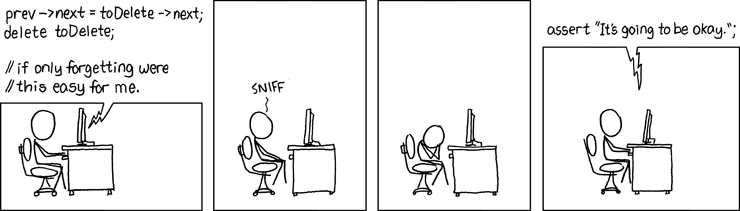
\includegraphics[width=\textwidth]{forgetting}
	\caption[]{\texttt{xkcd no.\ 379}}
	\label{fig:forgetting}
\end{figure}

\subsection{Pila}

La pila è una struttura dati \emph{dinamica}, \emph{lineare} in cui l'elemento rimosso dall'operazione di cancellazione è predeterminato, ed è quello che \enquote{è rimasto per meno tempo nell'insieme} (con strategia \textsc{LIFO}, \foreign{Last-In-First-Out}).

\begin{algorithm}[H]
	\caption[Specifica pila]{Specifica \textsc{Stack}}
	%&../preamble

% arara: pdflatex: { synctex: no }
% arara: latexmk: { clean: partial }
\ifstandalone
\begin{document}
\begin{algorithm}[H]
\fi

\Bool \stackEmpty \Comment*[r]{restituisce vero se la pila è vuota}
\stackPush{\Item \(v\)} \Comment*[r]{inserisce \(v\) in cima alla pila}
\Item \stackPop \Comment*[r]{estrae l'elemento in cima alla pila e lo restituisce al chiamante}
\Item \stackTop \Comment*[r]{legge l'elemento in cima alla pila}

\ifstandalone
\end{algorithm}
\end{document}
\fi

\end{algorithm}

Ogni volta che viene effettuata una chiamata a funzione si usa implicitamente una pila, che memorizza tutti i record di attivazione delle chiamate effettuate.
Sfrutteremo questo meccanismo implicito per visitare gli alberi, attraverso una visita in profondità.

Le pile possono essere implementate come:
\begin{itemize}
	\item liste bidirezionali, dove il puntatore punta all'elemento \textsf{top} (non utilizzate);
	\item tramite vettore, dove la dimesione è limitata quindi si crea un \foreign{overhead} più basso.
\end{itemize}

\begin{algorithm}[H]
	\caption{Struttura dati pila basata su vettore in pseudocodice}
	%&../preamble

% arara: pdflatex: { synctex: no }
% arara: latexmk: { clean: partial }
\ifstandalone
\begin{document}
\begin{algorithm}[H]
\fi
\begin{minipage}[t]{.45\textwidth}

% \BlankLine
\Item{} \(A\)	\Comment*[r]{elementi}
\Int \(n\)		\Comment*[r]{cursore}
\Int \(m\)		\Comment*[r]{dimesione massima}

\BlankLine
\tcp{crea una pila vuota}
\prototype{\Stack \stackConstructor{\Int dim}}{
	\Stack \(t =\) \new \Stack\;
	\(t.A =\) \new \Array{\Int}[0][dim-1]\;
	\(t.m = dim\)\;
	\(t.n = 0\)\;

	\BlankLine
	\Return \(t\)\;
}

\BlankLine
\tcp{leggi l'elemento in cima alla pila}
\prototype{\Item \stackTop}{
	\precondition{\(n > 0\)}

	\BlankLine
	\Return A[n]\;
}

% \vspace{10pt}
\end{minipage}\hfill%
\begin{minipage}[t]{.45\textwidth}
% \BlankLine
\tcp{restituisce \True se la pila è vuota}
\prototype{\Bool \stackEmpty}{
	\Return \(n \Equal 0\)
}

\BlankLine
\tcp{estrae l'elemento in cima alla pila e lo restituisce al chiamante}
\prototype{\Item \stackPop}{
	\precondition{\(n > 0\)}

	\BlankLine
	\Item \(t = A[n]\)\;
	\Decrement{n}\;

	\BlankLine
	\Return \(t\)
}

\BlankLine
\tcp{inserisce \(v\) in cima alla pila}
\prototype{\stackPush{\Item v}}{
	\precondition{\(n < m\)}

	\BlankLine
	\Increment{n}\;
	\(A[n] = v\)
}

\vphantom{0pt}

\end{minipage}
\ifstandalone
\end{algorithm}
\end{document}
\fi

\end{algorithm}

\begin{code}
	\captionof{listing}{Pila basata su vettore circolare in Java}
	\label{code:vector-stack}
	\pathinputminted{java}{VectorStack.java}
\end{code}

\clearpage
\subsection{Coda}

La coda è una struttura dati \emph{dinamica} \emph{lineare} in cui l'elemento rimosso dall'operazione di cancellazione è predeterminato, ed è quello che \enquote{è rimasto per più tempo nell'insieme} (con strategia, \textsc{FIFO}, \foreign{First-In-First-Out}).

\begin{algorithm}[H]
	\caption[Specifica coda]{Specifica \textsc{Queue}}
	%&../preamble

% arara: pdflatex: { synctex: no }
% arara: latexmk: { clean: partial }
\ifstandalone
\begin{document}
\begin{algorithm}[H]
\fi

\Bool \queueEmpty \Comment*[r]{restituisce vero se la coda è vuota}
\Item \queueInsert{\Item \(v\)} \Comment*[r]{inserisce \(v\) in fondo alla coda}
\Item \queueRemove \Comment*[r]{estrae l'elemento in cima alla coda e lo restituisce al chiamante}
\Item \queueTop \Comment*[r]{legge l'elemento in testa alla coda}

\ifstandalone
\end{algorithm}
\end{document}
\fi

\end{algorithm}

Nei sistemi operativi, i processi in attesa di utilizzare una risorsa vengono gestiti tramite una coda.
La politica \textsc{FIFO} è onesta (\foreign{fair}) rispetto l'ordine in cui i processi sono stati inseriti.

Le code possono essere implementate come:
\begin{itemize}
	\item liste monodirezionali, dove sono presenti due puntatori: uno alla testa (\foreign{head}) per l'estrazione, ed uno alla coda per l'inserimento;
	\item vettori circolari, il quale ha una dimensione limitata e crea un \foreign{overhead} più basso.
\end{itemize}

\begin{algorithm}[H][ht]
	\caption{Struttura dati coda basata su vettore circolare in pseudocodice}
	%&../preamble

% arara: pdflatex: { synctex: no }
% arara: latexmk: { clean: partial }
\ifstandalone
\begin{document}
\begin{algorithm}[H]
\fi
\begin{minipage}[t]{.45\textwidth}

\Item{} \(A\)	\Comment*[r]{elementi}
\Int \(n\)		\Comment*[r]{dimensione attuale}
\Int \(testa\)	\Comment*[r]{testa}
\Int \(m\)		\Comment*[r]{dimesione massima}

\BlankLine
\tcp{crea una cosa vuota}
\prototype{\Queue \queueConstructor{\Int dim}}{
	\Queue \(t =\) \new \Queue\;
	\(t.A =\) \new \Array{\Int}[0][dim-1]\;
	\(t.m = dim\)\;
	\(t.testa = 0\)\;
	\(t.n = 0\)\;

	\BlankLine
	\Return \(t\)\;
}

\BlankLine
\tcp{legge l'elemento in testa alla coda}
\prototype{\Item \queueTop}{
	\precondition{\(n > 0\)}

	\BlankLine
	\Return A[testa]\;
}

% \vspace{5pt}
\end{minipage}\hfill%
\begin{minipage}[t]{.45\textwidth}

% \BlankLine
\tcp{restituisce \True de la coda è vuota}
\prototype{\Item \queueEmpty}{
	\Return \(n \Equal 0\)\;
}

\BlankLine
\tcp{estrae l'elemento in testa alla coda e lo restituisce al chiamante}
\prototype{\Item \queueRemove}{
	\precondition{\(n > 0\)}

	\BlankLine
	\Item \(t = A[testa]\)\;
	\(testa = (testa+1) \bmod m\)\;
	\Decrement{n}\;

	\BlankLine
	\Return \(t\)\;
}

\BlankLine
\tcp{inserisce \(v\) in fondo alla coda}
\prototype{\Item \queueInsert}{
	\precondition{\(n < m\)}

	\BlankLine
	\(A[(testa+n) \bmod m]\) = \(v\)\;
	\Increment{n}\;
}

\vphantom{0pt}

\end{minipage}
\ifstandalone
\end{algorithm}
\end{document}
\fi

\end{algorithm}

\begin{figure}[hp]
\begin{code}
	\captionof{listing}{Coda basata su vettore in Java}
	\label{code:vector-queue}
	\pathinputminted{java}{VectorQueue.java}
\end{code}
\end{figure}

\ifsubfile
\end{document}
\fi
